\documentclass[11pt]{article}

% =========================================================================
% document style changes
% =========================================================================

\usepackage{amsmath}                    % AMS math packages
\usepackage{amssymb}                    %
\usepackage[]{graphpap}
\usepackage[T1]{fontenc}                % for \mathrm{}
\usepackage{courier}                    % for \texttt{}
\usepackage{bbm}                        % for \mathbbm{1} (indicator function)
\usepackage{booktabs}
\usepackage{graphicx}
\usepackage[font={small}]{caption}
\usepackage{subcaption}

%\setlength{\parskip}{\baselineskip}     % skip line following paragraphs
%\pagestyle{empty}                       % No page numbers
\setlength{\topmargin}{-.5in}
\setlength{\textheight}{9in}
\setlength{\oddsidemargin}{.125in}
\setlength{\textwidth}{6.25in}

\newcommand{\spc}{\vspace{0.25in}}      % Shortcut commands
\newcommand{\ds}{\displaystyle}         %\newcommand{\ds}[1]{\displaystyle{#1}}
\newcommand{\ra}{\rightarrow}
\DeclareMathOperator*{\argmax}{arg\!\max}
\DeclareMathOperator*{\argmin}{arg\!\min}

\begin{document}                        % This is where the document begins

\title{Improving Item-Item Similarity Estimation during Collaborative Filtering}
\author{Bill Chickering and Jamie Irvine\\
CS 399 with Anand Rajaraman\\
Stanford University}
\renewcommand{\today}{March 25, 2014}
\maketitle

\section*{Abstract}
\emph{Will write this when the paper is done}

\section*{Introduction}
Determining the similarity of two users or items is valuable for a
number of data-mining applications including recommender systems, product
assortment and differentiation, as well as branding. Collaborative filtering is
often used to exploit user-item rating data to make such estimates. This is 
typically done by computing the Pearson correlation or cosine similarity of 
vector representations of the users or items \cite{Su2009}. Given sufficient 
user-item rating data, this approach can be very effective. However, when the
rating data is sparse for one or both users/items, these metrics can
yield dramatic discrepancies compared to values computed with sufficient
data at a later point in time. In this report, we describe two novel techniques 
for estimating the true similarity of two users or items given limited common 
rating data.

To keep the present work focused, we confine ourselves to memory-based
collaborative filtering (CF) in which we work with a logical user-item matrix.
Each element of the matrix corresponds to a rating given by a particular user to a
particular item. Further, we choose to limit our analysis to item-item
similarity but note that these techniques should be equally effective at
improving user-user similarity estimation. In this representaion, an item is
a vector of the ratings it has received from all users. We now formalize the 
notion of item-item similarity. Two alternative models for the generation of 
user-item ratings are useful in arriving at two different definitions of the 
{\em true} item-item similarity.  

\section*{True Item-Item Similarity}

In the first model, we imagine users are randomly presented items to rate. Given 
a sufficient period of time, all users will eventually rate all items, creating
item vectors that contain provided ratings from all users. The true similarity 
in this model of {\em random} rating, denoted $TrueSimRand$, is then the vector 
product of two complete item vectors. That is, 
\begin{align}
TrueSimRand(A, B) = \frac{\sum\limits_{u\in U}
r_{u,A}r_{u,B}}{\sqrt{\sum\limits_{u\in U} r_{u,A}^2}
\sqrt{\sum\limits_{u\in U} r_{u,B}^2}},
\end{align}
where $A$ and $B$ are items, $U$ is the set of all users and $r_{u,I}$ is the 
rating given by user $u$ to item $I$.

In the second model, we imagine an unlimited supply of users, each of whom
chooses to rate a subset of items. The lack of a rating is now meaningful since
it indicates a lack of interest of a particular user for a particular item. This
is captured by the model through a default rating of zero \footnote{We address
the issue of rating bias and the precise meaning of a zero valued ratings later
in this report.}. At any point in time, we may estimate the true similarity in
this model of {\em preferential} rating, by computing the cosine similarity of
the two item vectors. Only in the limit of inifinite time does this estimate
converge to the true similarity, which we denote $TrueSimPref$.  That is,
\begin{align}
TrueSimPref(A, B) = lim_{t\to\infty}\frac{\sum\limits_{u\in U_{AB}}
r_{u,A}r_{u,B}}{\sqrt{\sum\limits_{u\in U_A} r_{u,A}^2}
\sqrt{\sum\limits_{u\in U_B} r_{u,B}^2}},
\end{align}
where $U_A$ is the set of users who have rated $A$, $U_B$ is the set of users
who have rated $B$, and $U_{AB}$ is the set of users who have rated both $A$ and
$B$.

\section*{Estimating Item-Item Similarity}

Of course, most systems will never acquire ratings from all users for all items.
Nor are we able to work in the limit of infinite time. We must therefore make
estimates of the true item-item similarity using only partial information. In
the case of $TrueSimPref$, the cosine similarity computed at any point in time
serves as a simple and obvious estimate. In using this estimate, we are treating
all missing ratings as intentionally omitted. When estimating $TrueSimRand$, the
choice of how to handle missing ratings is perhaps less obvious. Following the
convention of Breese et al. \cite{Breese1998}, we choose to use the Pearson
correlation \footnote{The Pearson correlation is traditionally characterized by
subtracting an expectation value from each dimension. This is only approximately
true in our case. We discuss the how we subtract rating biases later in this
report.} for this estimate, ignoring all ratings by users who have not rated
both items. To summarize, our naive estimates are
\begin{align}
PearSim(A, B) = \frac{\sum\limits_{u\in U_{AB}}
r_{u,A}r_{u,B}}{\sqrt{\sum\limits_{u\in U_{AB}} r_{u,A}^2}
\sqrt{\sum\limits_{u\in U_{AB}} r_{u,B}^2}}
\stackrel{?}{\approx} TrueSimRand(A, B)
\end{align}

\begin{align}
CosSim(A, B) = \frac{\sum\limits_{u\in U_{AB}}
r_{u,A}r_{u,B}}{\sqrt{\sum\limits_{u\in U_A} r_{u,A}^2}
\sqrt{\sum\limits_{u\in U_B} r_{u,B}^2}}
\stackrel{?}{\approx} TrueSimPref(A, B).
\end{align}


.....

Even worse, low confidence measurements of similarity are indistinguishable from
high confidence ones. In this paper, we develop and compare a number of methods
to produce more accurate estimates of similarity by incorporating confidence
into the similarity score.
 
Item-based collaborative filtering is a common technique for measuring the
similarity of two items. There are different forms of collaborative filtering.
For this paper, we use a traditional approach. Each item is represented as a
vector of ratings. The similarity score of two items is computed by measuring
the similarity of the two rating vectors.

There are a few ways to compute the similarity of two vectors. One approach is
to use Cosine-similarity, defined as the cosine of the angle between the two
vectors:
\begin{align}
CosSim(A, B) = \frac{\sum\limits_{u\in U_{AB}}
r_{u,A}r_{u,B}}{\sqrt{\sum\limits_{u\in U_{A}} r_{u,A}^2}
\sqrt{\sum\limits_{u\in U_{B}} r_{u,B}^2}}
\end{align}
where $U_{I}$ is the set of all users who rated item $I$, $U_{AB}$ is the set of
all users who rated both item $A$ and item $B$ and $r_{u,I}$ is the rating user
$u$ gave to item $I$. Another popular approach is to use Pearson correlation:
\begin{align}
PearsSim(A, B) = \frac{\sum\limits_{u\in U_{AB}}
r_{u,A}r_{u,B}}{\sqrt{\sum\limits_{u\in U_{AB}} r_{u,A}^2}
\sqrt{\sum\limits_{u\in U_{AB}} r_{u,B}^2}}
\end{align}

Other similarity functions exist, such as one-sided similarities, but Pearson
correlation and Cosine-similarity are the most popular and will be the two
measurements used in this paper. \footnotemark

\footnotetext{ Note that the difference between the two similarities is how they
handle unpaired ratings; that is ratings from a user who has not rated the other
item. Cosine-similarity considers the unknown rating from an unpaired rating to
be $0$ and then calculates the cosine of the two vectors. Pearson correlation
simply throws away all unpaired ratings and calculates the cosine of the two
modified vectors.}

Both similarity measurements primarily leverage information from common users,
that is users who have rated both items. Because of this, they perform well with
a large number common users, but give unreliable results when the items have few
common users. In an extreme case, if only one user has rated item $A$ and item
$B$, $PearsSim(A, B) = 1$ or $-1$. Not only is this unlikely to be an accurate
assessment of the true similarity of $A$ and $B$, it also gives the most extreme
results possible, without giving any indication that this is a low-confidence
calculation.

In this paper, we construct a more accurate similarity score by incorporating
the number of common users, $n$, into the similarity function. 

\section*{Problem}

The goal is to calculate a modified similiary function that leverages the number
of commonn users to better estimate the true similarity. Formally, we design
$ModSim$ such that for two items $A$ and $B$ with $n$ users in common

\begin{align}
ModSim(A, B, n) \approx TrueSim(A, B)
\end{align}
where $TrueSim$ is the true similarity of the two items. Of course, there is no
way to actually know the true similarity of two items, but for a good enough
similarity function, such as $PearsSim$ or $CosSim$ and a large enough $n$, we
can get a good estimate. Thus, we model $TrueSim$ as 
\begin{align}
TrueSim(A, B) = lim_{n\to\infty}Sim(A, B)
\end{align}
where $Sim$ is the most appropriate generic similarity function for the dataset.

Since $TrueSim$ dependends on the choice of $Sim$, we abstract away the details
of $Sim$ and use its output directly. In all, the goal is to construct $ModSim$
such that

\begin{align}
ModSim(Sim(A, B), n) \approx lim_{n\to\infty}Sim(A, B)
\end{align}

\section*{Linear Approach}
\subsection*{Probabilistic Model}

In our first approach, we model true and observed similarity probabilistically. For
this analysis, we can consider an abstact $TrueSim$ which ignores the details of 
$TrueSimRand$ or $TrueSimPref$. Similarly, we consider $Sim_{n}$ and $GoldSim$ to be
the generic observed similarity scores. Let $Y$ be a random variable representing 
the $TrueSim$ of a randomly chosen pair of items. Let $X_{n}$ be a random variable 
representing the $Sim_{n}$ of a pair of items when $n$ common users are observed.

We model $Y$ as a Normal distribution 
\begin{align}
Y \sim N(\mu, \sigma_{1}^2)
\end{align}
where $\mu$ and $\sigma_{1}^2$ are the average similarity score and the variance 
of similarity scores of all pairs of items, respectively. Since $X_n$ represents
a noisy reading of the true similarity $Y$, we model $X_n | Y=y$ as a Gaussian
error around $y$:
\begin{align}
(X_n | Y=y) \sim N(y, \sigma_{2, n}^2)
\end{align}

Note that $\sigma_{2, n}^2$ represents how noisy $Sim_n$ is as an estimation of
$TrueSim$ and therefore should decrease as $n$ increases. The probability
distribution of $X_n$ can be visualized in Figure 1.

\begin{figure}[!htbp]
    \centering
    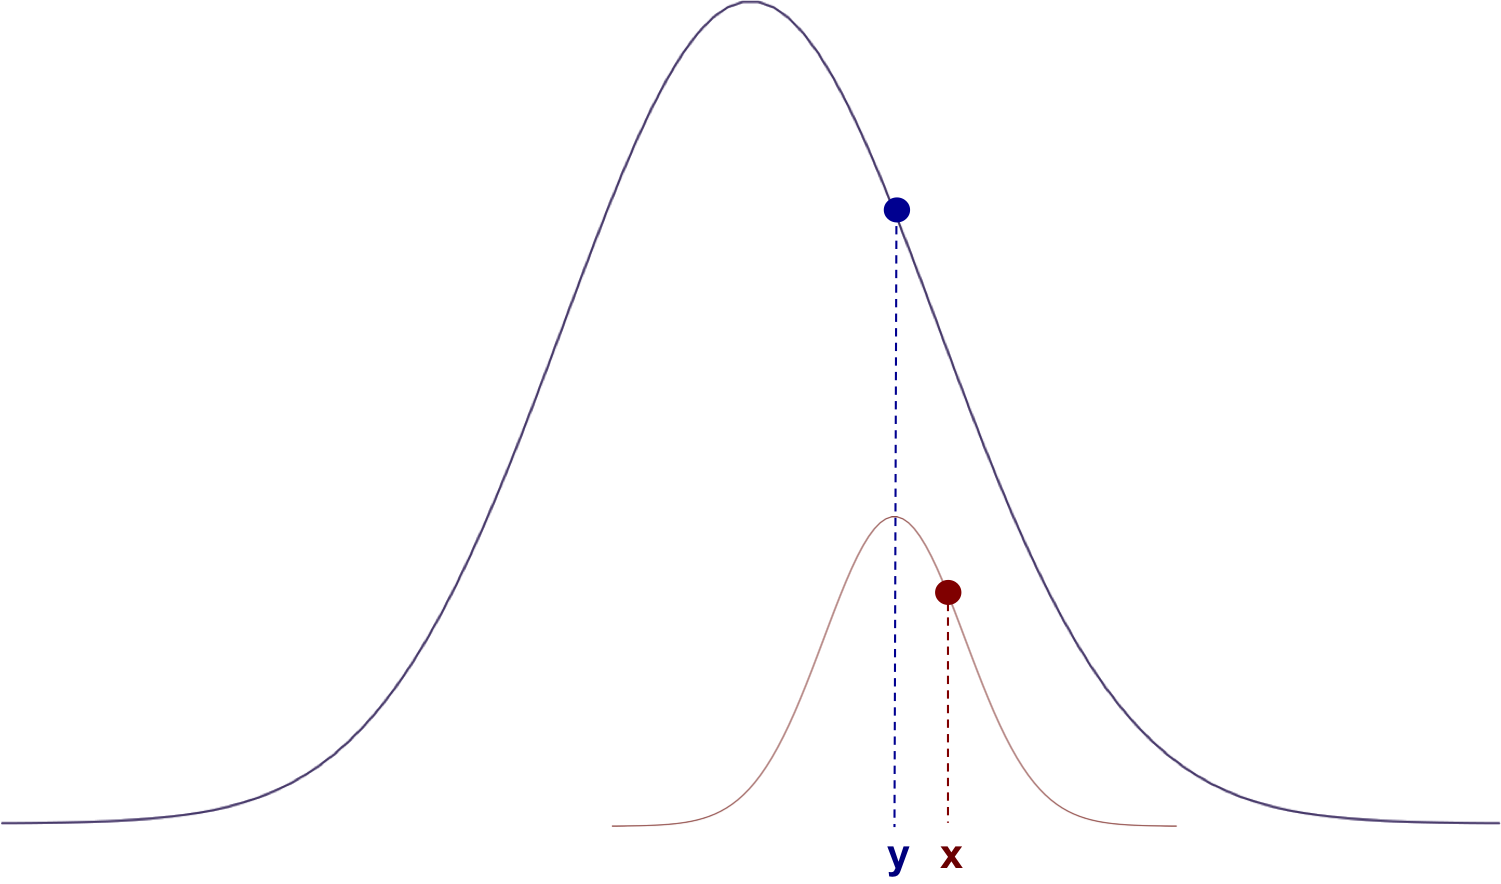
\includegraphics[width=0.7\textwidth]{twonormals.png}
	\caption{The blue curve represents $Y$, the distribution of true
    similarities between a random pair of items. The red curve represents $X|Y$,
    the observed similarity when a small number of common users exist.}
    \label{fig:two_normals}
\end{figure}

The problem of approximating the $TrueSim$ from $Sim_n$ can now be seen as
finding the value of $Y$ that most likely produced $X_n$. In other words we 
desire the Maximum Likelihood Estimate of $Y | X_n$:
\begin{align}
\hat{y} &= \argmax_yP(Y=y|X_n=x) 
\\&= \argmax_y\left[\frac{P(X_n=x | Y=y)P(Y=y)}{P(X_n=x)}\right]
\\&= \argmax_y\left[P(X_n=x|Y=y)P(Y=y)\right]
\\&= 
\argmax_y\left[\frac{1}{\sigma_{2,n}\sqrt{2\pi}}\exp{\left(\frac{-(x-y)^2}
{2\sigma_{2,n}^2}\right)}
\frac{1}{\sigma_{1}\sqrt{2\pi}}\exp{\left(\frac{-(y-\mu)^2}
{2\sigma_{1}^2}\right)}\right]
\\&= \argmin_y\left[\frac{(x-y)^2}{2\sigma_{2,n}^2} +
\frac{(y-\mu)^2}{2\sigma_{1}^2}\right]
\\&= \argmin_y\left[\left(\sigma_{1}^2+\sigma_{2,n}^2\right)y^2 - 
2\left(\sigma_{1}^2x+\sigma_{2,n}^2\mu\right)y\right]
\end{align}
We find the exact minimum by taking the derivative with respect to $y$ and
setting it to zero:
\begin{align}
\frac{d}{dy}\left[\left(\sigma_{1}^2+\sigma_{2,n}^2\right)y^2 - 
2\left(\sigma_{1}^2x+\sigma_{2,n}^2\mu\right)y\right]
&= 2\left(\sigma_{1}^2+\sigma_{2,n}^2\right)y - 
2\left(\sigma_{1}^2x+\sigma_{2,n}^2\mu\right) 
\\&= 0
\end{align}
This produces the following linear equation for \hat{y} in terms of x:
\begin{align}
\hat{y} &= \frac{\sigma_{1}^2x+\sigma_{2,n}^2\mu}{\sigma_{1}^2+\sigma_{2,n}^2}
\end{align}
which can be rewritten as:
\begin{align}
\left(\hat{y} - \mu\right) &= \frac{\sigma_{1}^2}{\sigma_{1}^2+\sigma_{2,n}^2}
\left(x-\mu\right)
\end{align}

The model suggests that there is a linear correlation between $X_n$ ($Sim_n$)
and $Y$ ($TrueSim$). Moreover, the best predicted $TrueSim$ is a linear 
combination of the mean and the observed similiarity. Since $\sigma_{2,n}^2$ is 
nonnegative, the slope is always less than or equal to one, meaning that the 
observed distance from $\mu$ (the average true similarity) overestimates the 
true distance. This is reasonable, since there is a prior that expects the true 
similarity to be around $\mu$.

The parameters $\mu$, $\sigma_{1}^2$, and $\sigma_{2,n}^2$ can be approximated 
using the method of moments over training data where there are enough common
users that $TrueSim$ can be approximated. This method requires approximating
$\sigma_{2,n}^2$ for every value of $n$ separately. To gain a more general 
model, we can model $\sigma_{2,n}^2$ as a function of $n$. Recall that 
$\sigma_{2,n}^2$ is the noisiness of the measurement $Sim$ about $TrueSim$ and $TrueSim = lim_{n \to
\infty}Sim$. Thus $Sim$ can be thought of as a sampling $n$ users from the
infinite set used to calculate $TrueSim$. Although $Sim$ may not be linear, we
the Central Limit Theorem motivates the intuition that the variance of $Sim$
would decrease as the $sqrt(n)$. Thus we model $\sigma_{2,n}^2$ as:
\begin{align}
\sigma_{2,n}^2 = \frac{\alpha}{\sqrt{n}},
\end{align}
yielding the single parameter model:
\begin{align}
\left(Y - \mu\right) = \frac{\sigma_{1}^2}{\sigma_{1}^2+\frac{\alpha}{\sqrt{n}}}
\left(X_n-\mu\right)
\end{align}
In terms of a modified similarity function, as desired earlier, we now have:
\begin{align}
ModSim(Sim, n) = \frac{\sigma_{1}^2}{\sigma_{1}^2+\frac{\alpha}{\sqrt{n}}}
\left(Sim-\mu\right) + \mu
\end{align}

\subsection*{Technique}
Based on this maodel, we try three different techniques to predict the true similarity from a
measured similarity. The techniques vary in their fidelity to the model. For
each, we limit our data to all pairs of items that have enough common users that
we can approximate $TrueSim \approx Sim$. Then we pick subsets of the common
users of various sizes $n$ and calculate $Sim_{n}$. With examples of $Sim$, $n$
and the resulting $TrueSim$, we can implement supervised learning.

The first technique is the least faithful to the model. It simply runs a number
of linear regressions between $Sim$ and $TrueSim$ for each $n$. This ignores the 
data-specific parameters $\mu$, $\sigma_{1}$ and $\sigma_{2,n}$ to find the best 
linear fit. It also treats each $n$ completely independently. This technique 
necessarilty has the lowest training error of all linear techniques, potentially 
at the risk of overfitting.

The second technique is more general. It approximates $\mu$ and $\sigma_{1}$
using the method of moments on the training data of all $TrueSim$ scores. Then,
$\sigma_{2,n}$ is also approximated using a method of moments on the training
data of all $Sim_n$ for each $n$ separately. Here $\sigma_{2,n}$'s are also
considered independently of each other.

The third and most general technique models $\sigma_{2,n}$ as a function of
$n$ using equation 19. As in the previous technique, $\mu$, $\sigma_{1}$ and each
$\sigma_{2,n}$ are approximated using the method of moments over the training
data. Then $\alpha$ is calculated that minimizes the sum of squared errors
between $\sigma_{2,n}^2$ and $\frac{\alpha}{\sqrt{n}}$. This $\alpha$ is used to
construct the three-parameter prediction function of equation 19.

\section*{Experiment}

\section*{Results}

\begin{figure}[!htbp]
    \centering
    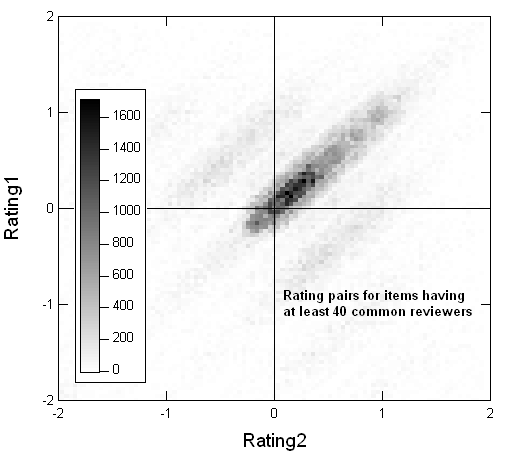
\includegraphics[width=0.7\textwidth]{RatingDist_40.png}
    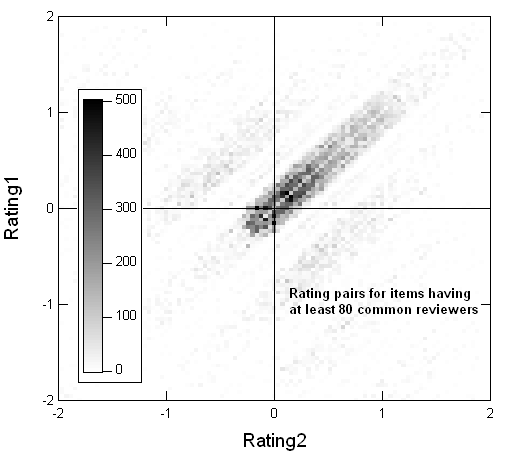
\includegraphics[width=0.7\textwidth]{RatingDist_80.png}
	\caption{Distribution of rating pairs by common reviewers for item pairs.
Top figure shows distribution for item pairs having at least 40 common
reviewers. Bottom figure shows distribution for item pairs having at least 80
common reviewers.}
    \label{fig:RatingDist}
\end{figure}

\begin{figure}[!htbp]
    \centering
    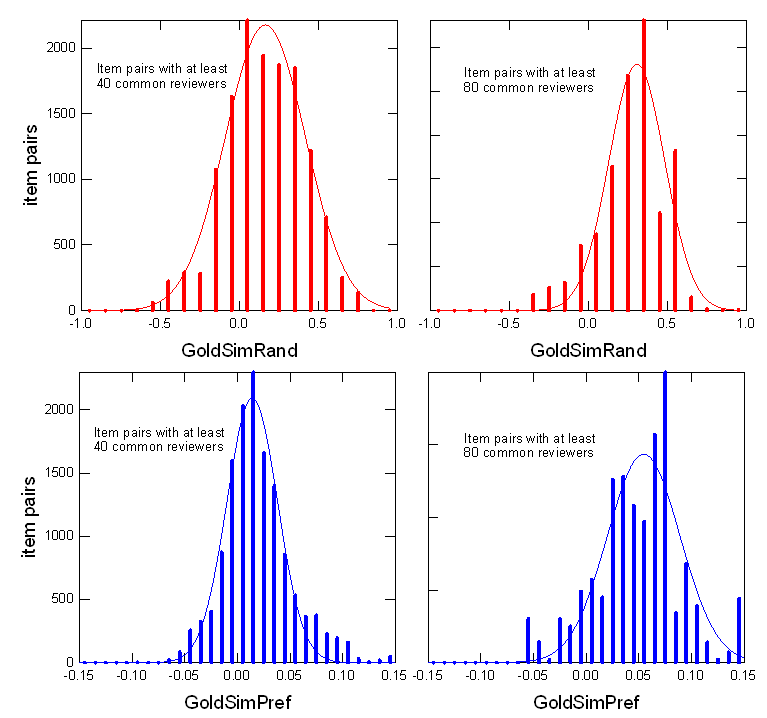
\includegraphics[width=1.0\textwidth]{Histograms.png}
	\caption{Histograms of {\em TrueSimR} (top) and {\em TrueSimP} (bottom) for
training datasets containing at least 40 common reviewers (left) and 80 common
reviewers (right).}
    \label{fig:Histograms}
\end{figure}

\begin{figure}[!htbp]
    \centering
    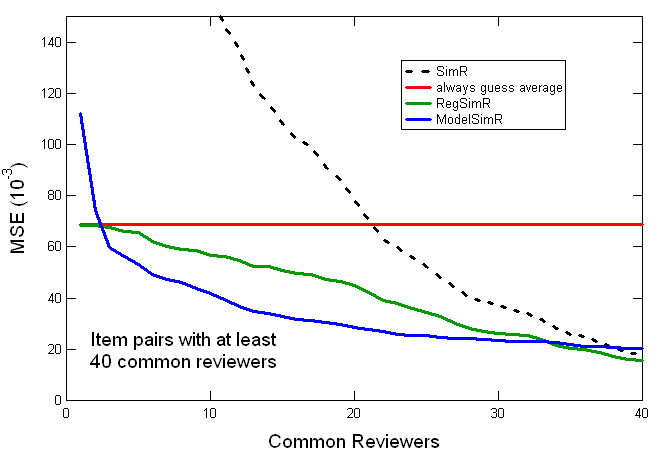
\includegraphics[width=0.9\textwidth]{MSE_SimR_40.png}
    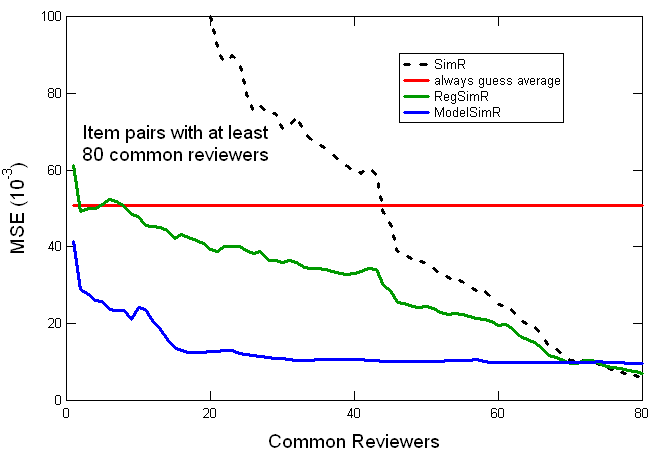
\includegraphics[width=0.9\textwidth]{MSE_SimR_80.png}
	\caption{Mean square error {\em vs} number of common reviewers, $n$, for
estimates of {\em TrueSimR} for item pairs ultimately having at least 40 common
reviewers (top) and 80 common reviewers (bottom). The dashed curve represents
{\em SimR} computed using only the ratings from the first $n$ reviewers. The
flat red line indicate the MSE that results from always guessing the average
{\em TrueSimR} from the training set. The green curve is {\em RegSimR} and the
blue curve is {\em ModelSimR}. }
    \label{fig:MSE_SimR}
\end{figure}

\begin{figure}[!htbp]
    \centering
    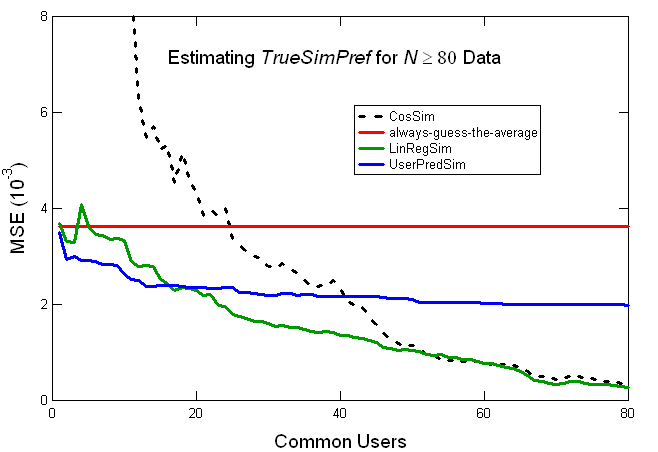
\includegraphics[width=0.9\textwidth]{MSE_SimP_80.png}
	\caption{Mean square error {\em vs} number of common reviewers, $n$, for
estimates of {\em TrueSimP} for item pairs ultimately having at least 80 common
reviewers. The dashed curve represents
{\em SimP} computed using only the ratings from the first $n$ reviewers. The
flat red line indicate the MSE that results from always guessing the average
{\em TrueSimP} from the training set. The green curve is {\em RegSimP} and the
blue curve is {\em ModelSimP}. }
    \label{fig:MSE_SimP}
\end{figure}

\section*{Conclusion}
\begin{thebibliography}{9}

\bibitem{Su2009}
    Xiaoyuan Su and Taghi M. Khoshgoftaar.
    ``A Survey of Collaborative Filtering Techniques.''
    \emph{Advances in Artificial Intelligence.} vol. 2009,
    Article ID 421425, 19 pages, 2009. doi:10.1155/2009/421425
\bibitem{Breese1998}
    Breese, John S., David Heckerman, and Carl Kadie, 
    ``Empirical analysis of predictive algorithms for collaborative filtering.'' 
    \emph{Proceedings of the Fourteenth conference on Uncertainty in artificial intelligence.}
    Morgan Kaufmann Publishers Inc., 1998.
\bibitem{Lemire1998}
    Daniel Lemire and Anna Maclachlan.
    ``Slope One Predictors for Online Rating-Based Collaborative Filtering.''
    \emph{SDM.} Vol. 5, 2005.

\end{thebibliography}

\end{document}
